\chapter{Hunter: Tracing Anycast}
\label{ch:hunter}

It is clear that anycast communications, with their "natural" behaviour, impose severe risks to privacy, data protection, and data sovereignty. This thesis has the objective of clarifying the severity of this risk, and to achieve this, the first step is to be able to track anycast paths, or at least the physical destination of these types of communications. For that purpose, I developed a method capable of tracking the multiple destinations to which anycast IP could send data, given the origin. To achieve this objective, the method uses different ICMP measurements, including traceroute \cite{Traceroute8Page} and ping \cite{Ping8Page}, to track the path followed by the communication. Because the complete path can be tracked, every different path an anycast communication follows is suitable for identification. Finally, I implemented an automation of this method named Hunter, which is open source and can be used by other researchers in their work. 

The developed method consists of 3 steps that are carried out sequentially. First, it traces the different network elements which compose the route to the destination. It is crucial for our purpose to have the correct information about the last hop, the one just before reaching the destination. The second step is multilateration. Several vantage points are selected with the condition of being close to the last hop. From these vantage points, multilateration is carried out, obtaining the area where the destination physical location must be. At last, it determines the city and country within the destination are geolocated. If the method is applied with Hunter, you should expect the output to be the city and the country where the destination server is located, or 'Indeterminate' if a valid result cannot be obtained. We detail each step in the following sections.

\begin{figure}
    \centering
    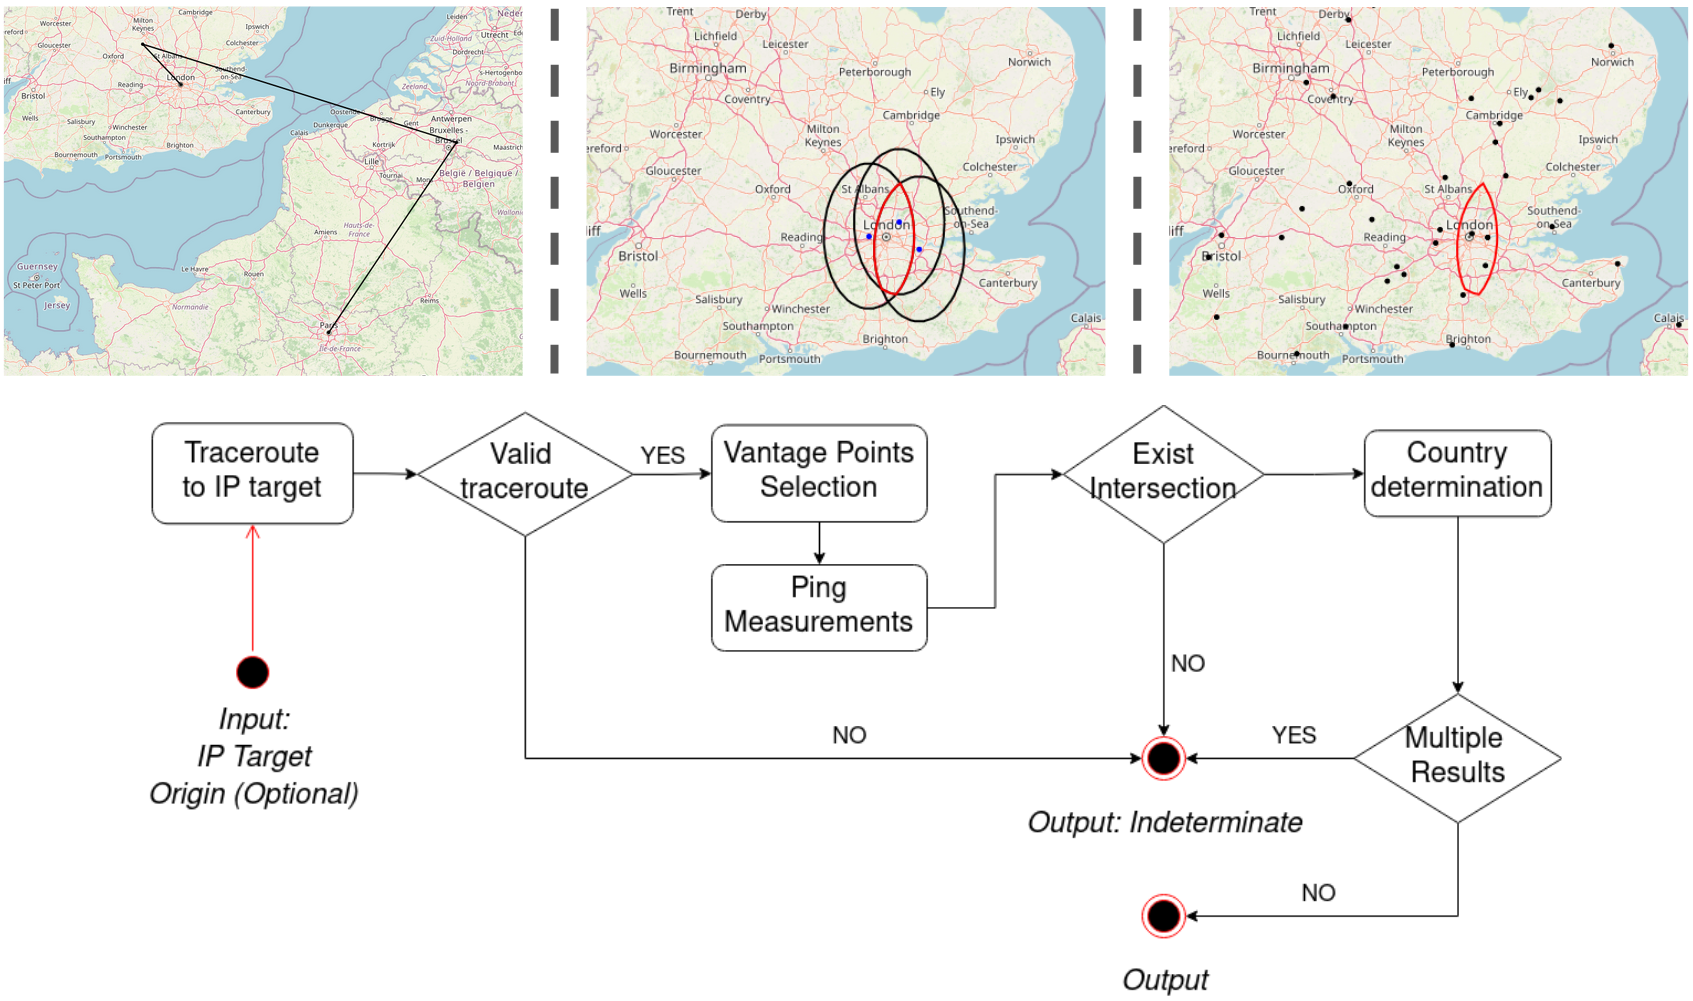
\includegraphics[width=\textwidth]{figures/hunter_steps.png}
    \caption{Hunter steps to determine the destination country for anycast communications.}
    \label{fig:hunter_steps}
\end{figure}

\section{Tracing Path}\label{sc:hunter_tracing_path}

The first step is being capable of tracking the complete path of the anycast communication. To this end, the traceroute tool is used to obtain the network hops, (network elements traversed by the packets, as shown in Figure \ref{fig:hunter_steps} (left). Traceroute is a network tool commonly used by network administrators for tasks like connectivity tests, validating appropriate routing, and more. In my case, I use this tool to obtain the different machines involved in the path followed by the anycast packets.

This tool works only at the IP level, which is appropriate for the research case. By default, traceroute input is an IP address, which being the one to be tracked. From the origin network element, three packets are sent to the destination IP with a Time To Live (TTL) of 1, which means these packets are going to be discarded by the first network element encountered. The network element which discard these packets responds with an ICMP "time exceeded" reply, from which it is possible to retrieve the IP of the replying network element. This strategy is repeated, increasing the TTL value until the maximum, 30 by default. By applying this strategy, the host obtains the path followed to the destination with the actual network conditions. Traceroute is a very powerful tool but has some limitations and does not always produce a usable result with the followed path.

\subsection{Traceroute limitations}

In order to understand the limitations of traceroute, it is essential to know which type of packets are sent and their characteristics. First of all, the packet length is defined as an input to the tool, but almost always the default of 60 bytes for IPv4 and 80 bytes for IPv6 is used. This packet length enables fast processing in routers and other network elements, almost reducing the processing time to just the routing decision making. This condition does not impose a specific limitation on traceroute.

However, the second defining characteristic of the packets used to measure could be problematic. There are three different protocol options: UDP, ICMP, and TCP. The default and traditional protocol used is UDP. Packets sent with UDP are directed to a port, in the Linux implementation 33434, that has no usage in the common network services deployed on the Internet. This type of packet could be filtered by firewalls, producing a path limited to the network element prior to the firewall. These types of results are discarded by Hunter. If ICMP packets are selected, then standard ICMP echo packets are used, the same as those used for ping. These packets could have an advantage over UDP since ICMP packets are usually not filtered by network elements, as they are used by the owners of these elements for diagnosis. However, some very restrictive organisations do not reply to this protocol, or the ICMP packets are discarded. Finally, when TCP packets are selected, they are sent to the destination port 80, the same one used for HTTP. Since the HTTP port is rarely filtered, these TCP packets are not filtered either. The major side effect that TCP has is to control the connection status since the TCP protocol is designed to maintain the connection between the implied agents. Nevertheless, the actual implementation of this tool resolves this issue without resulting in multiple TCP open connections. Although TCP could be the most convenient protocol, this is not true in all cases. Since the TCP option is used, the packets sent are treated as HTTP. Therefore, the routing could be different, with fewer intermediate network elements or network elements behaving differently in various ways because of a quality of service policy.

\hugo{This example is here just to keep it but I do not know what format use.} The following terminal responses are an example of this behaviour.

\begin{verbatim}
hugopascual@hp-shared:~$ sudo traceroute -T google.com
traceroute to google.com (142.251.142.142), 30 hops max, 60 byte packets
 1  swcdc30-polaris.dit.upm.es (138.4.11.131)  2.367 ms  2.733 ms  3.127 ms
 2  pfsense1.dit.upm.es (138.4.5.4)  0.145 ms  0.107 ms  0.163 ms
 3  r7000-ext.dit.upm.es (138.4.0.1)  0.491 ms  0.450 ms  0.461 ms
 4  192.168.214.18 (192.168.214.18)  0.755 ms  0.729 ms 192.168.214.19 (192.168.214.19)  0.749 ms
 5  * * *
 6  192.168.201.3 (192.168.201.3)  1.326 ms  1.653 ms  1.943 ms
 7  lcmada-ag-in-f14.1e100.net (142.251.142.142)  1.924 ms  1.598 ms  1.717 ms
hugopascual@hp-shared:~$ sudo traceroute google.com
traceroute to google.com (142.251.142.142), 30 hops max, 60 byte packets
 1  swcdc30-polaris.dit.upm.es (138.4.11.131)  2.420 ms  2.734 ms  3.150 ms
 2  pfsense1.dit.upm.es (138.4.5.4)  0.500 ms  0.456 ms  0.427 ms
 3  r7000-ext.dit.upm.es (138.4.0.1)  0.525 ms  0.547 ms  0.551 ms
 4  192.168.214.19 (192.168.214.19)  0.754 ms  0.829 ms  0.796 ms
 5  * * *
 6  192.168.201.3 (192.168.201.3)  3.165 ms  2.953 ms  3.038 ms
 7  172.17.0.13 (172.17.0.13)  1.294 ms  1.224 ms  1.501 ms
 8  193.145.14.233 (193.145.14.233)  1.507 ms  1.242 ms  1.250 ms
 9  redimadrid-ppal.ethtrunk14-103.ciemat.rt2.mad.red.rediris.es (130.206.212.105)  1.591 ms  2.231 ms  2.172 ms
10  ciemat-rt2.ethtrunk1.telmad.rt1.mad.red.rediris.es (130.206.245.25)  2.082 ms  2.868 ms  2.395 ms
11  * * *
12  108.170.252.225 (108.170.252.225)  4.232 ms  4.167 ms 108.170.252.213 (108.170.252.213)  2.073 ms
13  142.250.232.11 (142.250.232.11)  2.125 ms 142.250.232.27 (142.250.232.27)  2.083 ms 142.250.232.11 (142.250.232.11)  2.042 ms
14  lcmada-ag-in-f14.1e100.net (142.251.142.142)  3.276 ms  1.706 ms  1.733 ms
hugopascual@hp-shared:~$ sudo traceroute -I google.com
traceroute to google.com (142.251.142.142), 30 hops max, 60 byte packets
 1  swcdc30-polaris.dit.upm.es (138.4.11.131)  2.700 ms  3.139 ms  3.589 ms
 2  pfsense1.dit.upm.es (138.4.5.4)  0.138 ms  0.136 ms  0.134 ms
 3  r7000-ext.dit.upm.es (138.4.0.1)  0.503 ms  0.535 ms  0.533 ms
 4  192.168.214.18 (192.168.214.18)  0.803 ms  0.989 ms  0.987 ms
 5  * * *
 6  172.17.0.14 (172.17.0.14)  0.978 ms  0.838 ms  0.826 ms
 7  172.17.0.13 (172.17.0.13)  1.083 ms  0.845 ms  0.891 ms
 8  193.145.14.233 (193.145.14.233)  0.995 ms  0.872 ms  0.878 ms
 9  redimadrid-ppal.ethtrunk14-103.ciemat.rt2.mad.red.rediris.es (130.206.212.105)  1.557 ms  1.673 ms  1.663 ms
10  ciemat-rt2.ethtrunk1.telmad.rt1.mad.red.rediris.es (130.206.245.25)  2.253 ms  2.069 ms  2.003 ms
11  * * *
12  108.170.252.225 (108.170.252.225)  2.420 ms  3.589 ms  3.091 ms
13  142.250.232.27 (142.250.232.27)  2.425 ms  2.415 ms  2.435 ms
14  lcmada-ag-in-f14.1e100.net (142.251.142.142)  2.242 ms  2.236 ms  2.338 ms
\end{verbatim}

\begin{figure}
    \centering
    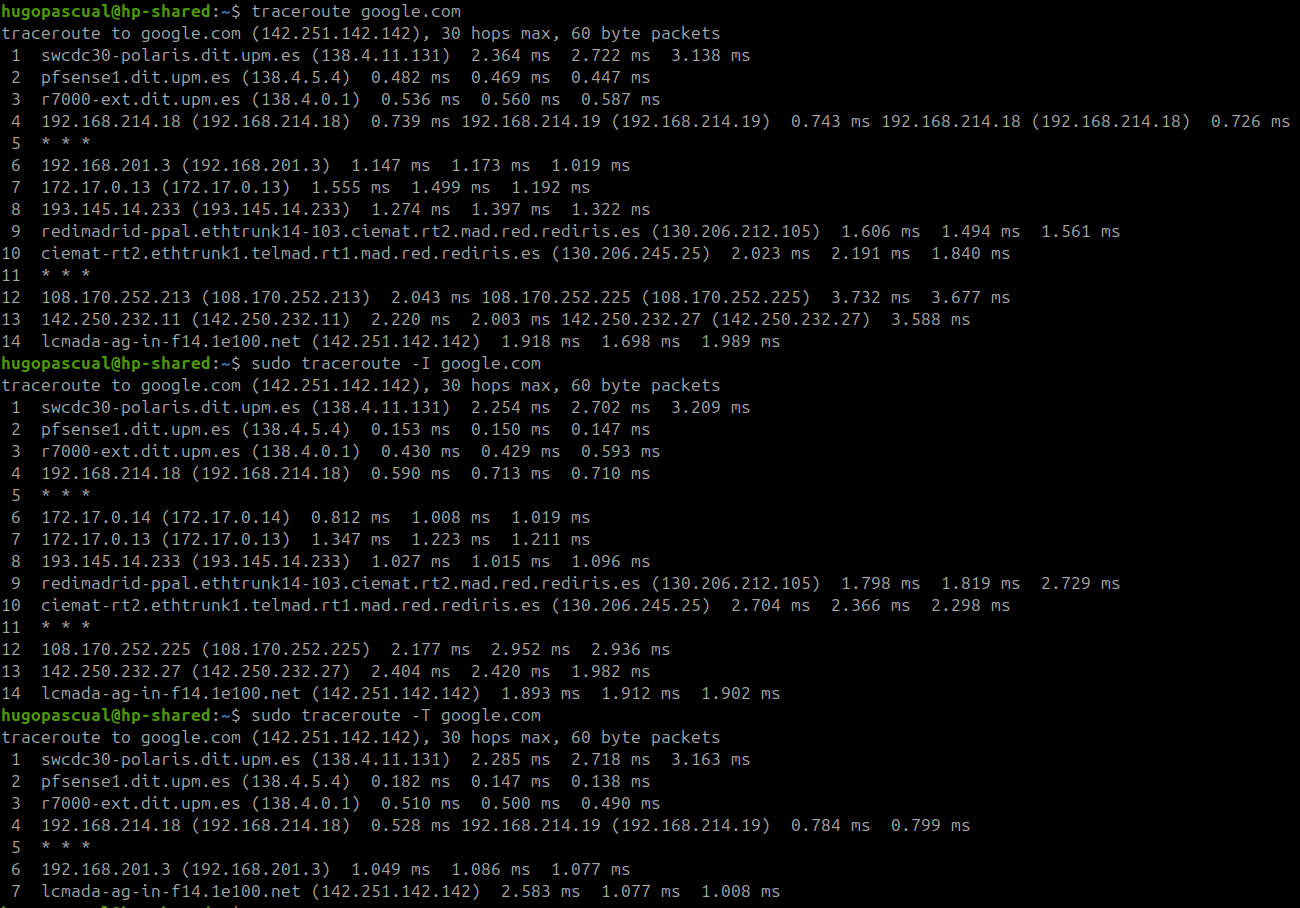
\includegraphics[width=\textwidth]{figures/traceroute_protocols_examples.png}
    \caption{Example of traceroute execution using all three different protocols.}
    \label{fig:traceroute_protocols_examples}
\end{figure}

Getting partial results with the packets being filtered and not arriving at the destination is not the only issue encountered when using traceroute. The other behaviour that is mandatory to take into account is the multipathing during a measurement. As described above, more than one packet is sent with the same TTL from the host. These multiple packets could follow the same path, or they could separate, reaching the destination through different network elements. This situation could result in two different outcomes: the path length is the same or different. Dealing with anycast IP addresses, both situations could mean that multiple anycast replicas were involved in the communication. Because of this, all the possible paths are treated as different results, and the Multilateration phase \ref{sc:hunter_multilateration} and the Country Determination phase \ref{sc:hunter_country_determination} must be executed multiple times.

\hugo{This behaviour is the one in the last experiment done. In the first version we take the decision to trim different "strange results" instead of treating them separately. I must review how to integrate both because the validation should be valid as we separate "strange results" in the last version similarly to the trim decisions we make in the first version.}

\section{Multilateration}\label{sc:hunter_multilateration}

Once a valid path is selected, the multilateration phase starts. First of all, the last hop of the path is obtained and validated. This last hop is the network element just before the destination. In most cases, it is a router, but it could also be a load balancer or another element designed to control and route packets to the destination server. The last hop is the nearest network element to the destination in network terms and usually in physical distance. This router IP is geolocated using commercial databases, and these coordinates are used as the centre for selecting vantage points. The selection of the vantage points is made randomly within a given distance from the last hop location. A measurement is taken using ping to the destination IP address to obtain the round trip time (RTT) from every vantage point. Knowing the location of the probes, the RTT to reach the destination from each probe, and the propagation speed of the packets, the maximum distance travelled by each packet can be computed. A circumference can be drawn for each probe, as we know their location and the maximum distance travelled by the packets they send to the destination. The destination server should be within the overlapping area of the circumferences.

The behaviour previously described is the common one when the assumptions and conditions are valid. However, the assumptions are not always valid, and there are many control decisions that should be made which affect the result and the performance of the method. The first assumption is that the last hop network element is a router or any kind of specific routing element, like a load balancer. Routers in the Internet should not be assigned anycast IPs because that situation could provoke routing problems, and it does not fit into the responsibility and use of a router. For that reason, routers use unicast IP addresses. These routers' unicast addresses are well geolocated by commercial geolocation databases, as routers are not network elements that change locations frequently, and their IPs are not assigned dynamically, as is the case with cloud servers. Nevertheless, the last hop element could have an anycast IP because it is not a router like element, which provokes an invalid result. In this case, the path is discarded.

The second assumption is that the last hop and the destination are physically proximate. This behaviour is the usual one but is not mandatory, and the contrary case should be controlled. This situation could result in a different physical destination for the vantage points selected for the ping measurement. In this case, the overlapping area is too large to be considered valid, or there is no overlapping area. Once this situation occurs, the path is discarded, and no results are produced. 

Hunter allows setting the number of vantage points, both desired and minimum, to be used and their maximum distance to the last hop. In contexts where the transmission speed is deterministic, three vantage points would be enough to geolocate a target, i.e., trilateration. However, we can only set an upper boundary on the transmission speed; thus, we use several vantage points to improve the accuracy of the location. Using more vantage points generally results in smaller overlapping areas but at the cost of computing time (to set up the vantage points, run the measurements, and obtain the results). Using larger distances when selecting the probes also reduces the overlapping areas, up to a point when far-away probes send their packets to a different anycast instance closer than the targeted one. Our empirical results show that using 7 probes and a distance of 20 kilometres provides a better trade-off between performance and accuracy.

\section{Country determination}\label{sc:hunter_country_determination}

Once the overlapping area of the circumferences has been obtained, an analysis is performed to establish the city and the country where the destination server is located. Anycast IP addresses are used in online services to distribute the load among several distant locations and improve response times. For this reason, they are usually located near urban centres. Taking this into account and inspired by previous work in the field \cite{Cicalese2016Latency-BasedSets}, we used a list of the world's main airports as approximate locations of the cities where the different anycast instances can be found. This argument is reinforced, e.g., by CDNs such as Cloudflare using the IATA code of the nearest airport as an identifier of the city where a given server is located.

Hunter's analysis begins by searching for airports within the overlapping area. When performing this search, there are three possible results: no airport in the area, one single airport in the area, or several airports in the area. In the first case, the centroid of the overlapping area is calculated, and the closest airport to that point is used as a reference airport. For each airport found, the associated cities and corresponding countries are retrieved. In scenarios with only one airport, there will be only one city and one country, which will be Hunter output. If multiple airports are obtained, then the associated countries are checked. If all airports belong to the same country, this will be the final result. Otherwise, the result will be \textit{Indeterminate}.

\section{RIPE Atlas}\label{hunter_ripe_atlas}

The network measurements described in the previous sections could theoretically be performed from a single personal computer. However, such an approach would severely limit the geographic diversity of the measurements, since the location of the measurement host would remain fixed. As the objective of Hunter is to infer the potential geographic destinations of anycast communications on a continental and global scale, it is necessary to employ a distributed measurement infrastructure that provides geographically diverse vantage points.

For this purpose, the implementation of Hunter relies on RIPE Atlas \cite{HomeAtlas}, a large-scale Internet measurement platform composed of thousands of distributed probes deployed worldwide. RIPE Atlas enables researchers and network operators to perform active measurements such as ping, traceroute, DNS, TLS, HTTP, or NTP from multiple geographic locations. These probes are hosted by volunteers, organisations, universities, Internet Service Providers (ISPs), and research institutions, providing broad visibility into the global Internet infrastructure.

The platform is publicly accessible and community-driven, allowing participants to contribute probes and perform measurements through a credit-based system. RIPE Atlas is maintained by the RIPE Network Coordination Centre (RIPE NCC), the Regional Internet Registry responsible for Europe, the Middle East, and parts of Central Asia. As one of the major organisations involved in Internet coordination and infrastructure management, RIPE NCC provides a reliable and widely adopted platform for Internet-scale measurement studies.

Several alternative Internet measurement platforms exist, including Ark CAIDA \cite{ArkCAIDA}, perfSONAR \cite{PerfSONAR}, and PlanetLab \cite{HomePlanetLab}. However, RIPE Atlas was selected for this work due to its large number of active probes, extensive geographic coverage, measurement flexibility, and widespread adoption within the network research community.

These characteristics make RIPE Atlas particularly suitable for the objectives of Hunter, as the methodology requires executing traceroute and latency measurements from multiple distributed vantage points in order to estimate the geographic regions potentially reached by anycast communications.

\section{Validation}\label{sc:hunter_validation}

\hugo{This validation is not very rigid, everyone that reads it is going to comply about: the use of a VPN and why reducing the validation only to Europe. Furthermore, it needs to explicitly present the metrics of the different work scenarios: checking last hop IP if anycast or not and the approximation of the last hop geolocation to the destination one. At last I need to include all the parameters used for the traceroute, the ones explained in traceroute section.}

The method presented and its software implementation, Hunter, have been validated in a real world scenario to assure its correctness and accuracy and precision statistics. For that purpose, we have used two anycast IP addresses of the Cloudflare CDN to validate Hunter. The HTTP responses from these IP addresses include a header, CF-RAY, with the IATA code which identifies the closest airport to the server, thus revealing its location. The first address, 192.5.5.241, belongs to a root DNS service, and the second one, 104.16.123.96, serves Cloudflare's official website.

The tests executed Hunter using the two chosen addresses as the destination. Right before executing Hunter, an HTTP request was made to the destination to compare Hunter's output with the actual destination. This obtained the ground truth to assess Hunter's output. Since our final goal is to check compliance with the GDPR requirements for international transfers of personal data, we have carried out the tests from nearly all European Economic Area (EEA) countries. To this end, we used a Virtual Private Network (VPN) service to simulate our location (communication source). In particular, each validation with the two destination addresses has been executed from each country belonging to the EEA, except for Liechtenstein, due to the VPN not providing an exit node in that country.

For the assessment, we compared the location of the target server obtained with Hunter and the location declared by the target server in the HTTP request headers. We can obtain 3 possible results: Indeterminate, Positive and Negative. Indeterminate when the method encounters one situation that prevents it from advancing as described in previous sections; Positive if Hunter output equals the one declared by the server; and Negative if Hunter output is different from the one declared by the server. 

Hunter achieves a noteworthy 97.67\% precision and 78.09\% accuracy in determining the destination location. The precision is defined as the ratio between the number of Positives and the sum of Positives and Negatives obtained. The accuracy is defined as the ratio between the number of Positives and the total number of results obtained in that test, whether Positive, Negative, or Indeterminate. These results show Hunter's reliability in identifying the target country of anycast communications.

Building upon Hunter's evaluation, we conducted a comparative analysis with a straightforward approach to anycast location identification, which involves geolocating the IP of the last hop using the IPinfo service. The evaluation of the straightforward approach indicates it can identify more countries (+0.44\%) at the cost of increasing the Negative results (+13.72\%). We aim to assess legal compliance, so we should favor soundness over completeness. Thus, Hunter identifies cross-border transfers while minimizing the occurrence of erroneous identifications, assuming that it may occasionally lead to the omission of certain transfers in favor of ensuring reliability.

\subsection{International Transfers during Validation}

\begin{figure}
    \centering
    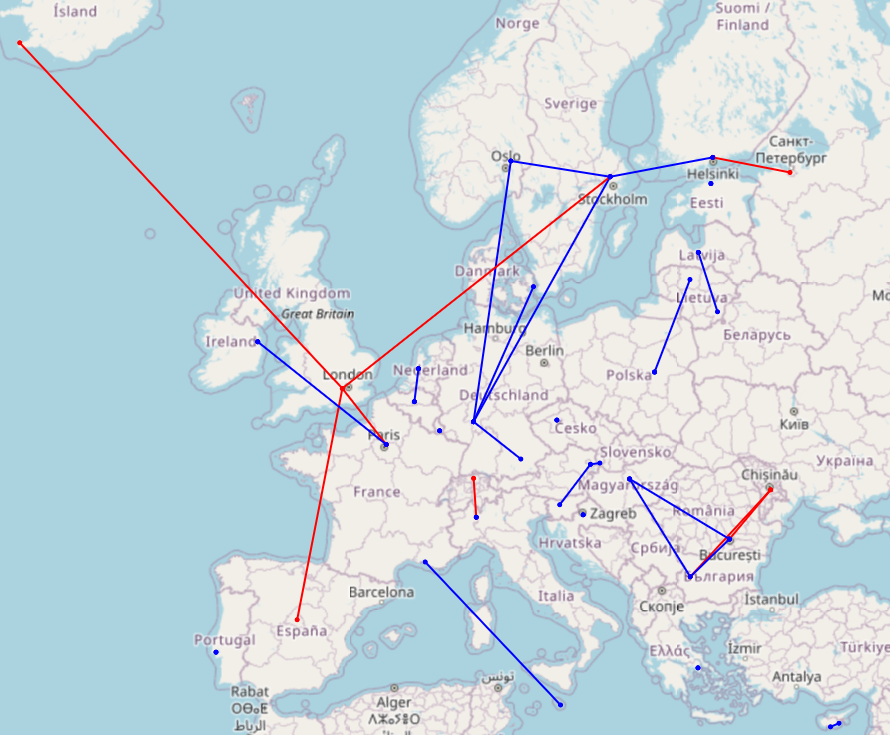
\includegraphics[width=\textwidth]{figures/validation_flows.png}
    \caption{Data flows obtained during Hunter validation (in red, flows crossing the EEA borders) with target 192.5.5.241.}
    \label{fig:validation_flows}
\end{figure}

The data flows captured during Hunter validation show many destinations outside the EEA. As shown in Figure \ref{fig:validation_flows}, the non-EEA destination countries for the IP address 192.5.5.241 are the United Kingdom, Switzerland, Moldova, and Russia. We have observed three patterns for these communications: recurrent, frequent, and episodic. Recurrent cross-border data transfers can be seen in countries such as Spain or Iceland, where all the communications to the target address have the United Kingdom as the destination. Frequent cross-border communications are seen, e.g., in Finland, where the destinations are equally distributed between Sweden and Russia. Finally, we observed episodic communications from Italy to Switzerland and from Sweden to the United Kingdom. This indicates that the destination can vary significantly due to the punctual state of the network at the time of the communication. 

Analyzing in detail the Negative results for each origin country, we found that 94.12\% of the Negative results (48 out of 51) were concentrated in Norway and Finland, with an accuracy of 50.72\% and 80.28\%, respectively. However, we also observed that systematically repeating the measurements over time solved this problem. Indeed, Hunter achieves absolute (100\%) accuracy if, when applied over a period of time, only those results with sufficient statistical significance are marked as valid. Our empirical results show that when a country appears in the results over 5\% of times, it can be considered a valid result.

